\documentclass{../tufte-handout}

\title{Lecture 1: Why Probabilistic Programming?\thanks{CS7470 Fall 2023: Foundations of Probabilistic Programming.}}

\author[]{Steven Holtzen\\s.holtzen@northeastern.edu}

%\date{28 March 2010} % without \date command, current date is supplied

%\geometry{showframe} % display margins for debugging page layout
\setcounter{secnumdepth}{1}

\usepackage{graphicx} % allow embedded images
  \setkeys{Gin}{width=\linewidth,totalheight=\textheight,keepaspectratio}
  \graphicspath{{graphics/}} % set of paths to search for images
\usepackage{amsmath,amssymb,amsthm}  % extended mathematics
\usepackage{booktabs} % book-quality tables
\usepackage{units}    % non-stacked fractions and better unit spacing
\usepackage{multicol} % multiple column layout facilities
\usepackage{lipsum}   % filler text
\usepackage{fancyvrb} % extended verbatim environments
  \fvset{fontsize=\normalsize}% default font size for fancy-verbatim environments
\usepackage{listings}
\usepackage{tikz}
\usepackage{mathpartir}
\usepackage{subcaption}
\usepackage{mdframed}
\usepackage{epigraph}
\usepackage{enumitem}
\usepackage{stmaryrd}

\usetikzlibrary{shapes.geometric}


\usepackage[ruled,linesnumbered]{algorithm2e}
\SetKwComment{Comment}{/* }{ */}
\newcommand{\indep}{\perp \!\!\! \perp}

\tikzset{
  treenode/.style = {shape=rectangle, rounded corners,
                     draw, align=center,
                     },
  root/.style     = {treenode, font=\Large, bottom color=red!30},
  env/.style      = {treenode, font=\ttfamily\normalsize},
  dummy/.style    = {circle,draw}
}

% tikz
\usetikzlibrary{patterns,calc,backgrounds}


% TIKZ
\tikzstyle{nnf}=[
  >=stealth,font=\small,auto,scale=0.7,every node/.style={scale=0.7}
]
\tikzstyle{extnode}=[
  draw,circle,inner sep=2pt,fill=white
]

\tikzstyle{leafnode}=[
  draw,fill=gray!20,inner sep=3.5pt
]
\tikzstyle{constnode}=[
  draw,fill=white,inner sep=3.5pt
]
\tikzstyle{label}=[
  fill=white,inner sep=2.5pt
]

\tikzstyle{acarrow}=[
    decoration={markings,mark=at position 1 with {\arrow[scale=0.6]{>}}},
    postaction={decorate},
    shorten >=0.4pt,
    >=latex,
    line width=0.1
]

\tikzstyle{bnarrow}=[
    decoration={markings,mark=at position 1 with {\arrow[scale=1.5]{>}}},
    postaction={decorate},
    shorten >=0.7pt,
    >=latex,
    line width=0.3
]
\tikzstyle{bayesnet}=[
  >=latex, thick, auto
]
\tikzstyle{bnnode}=[
  draw,ellipse,minimum size=7mm,inner sep=1pt,font=\small
]
\tikzstyle{cpt}=[
  font=\footnotesize
]

\tikzstyle{graph}=[
  >=stealth,font=\small,auto,scale=1,every node/.style={scale=1}
]
\tikzstyle{node}=[
  draw,circle,inner sep=3pt,fill=white
]

% BDDs

\tikzstyle{bdd}=[
  >=latex, thick, >=stealth, font=\small,auto,scale=0.9,every node/.style={scale=0.9}
]
\tikzstyle{bddnode}=[
  draw,circle,inner sep=0pt,fill=white,minimum size=5.5mm
]

\tikzstyle{bddtriangle}=[
  draw, regular polygon, regular polygon sides = 3,inner sep=1pt,fill=white,minimum size=5.5mm
]

\tikzstyle{highedge}=[
    line width=0.9
]
\tikzstyle{lowedge}=[
    line width=0.9,dotted
]
\tikzstyle{bddterminal}=[
  draw,fill=gray!20,inner sep=2.5pt, font=\small
]

\lstdefinestyle{compact}{
  \ttfamily\tiny
}


\usetikzlibrary{positioning}

\newtheorem{theorem}{Theorem}
\newtheorem{definition}{Definition}
\newtheorem{conjecture}{Conjecture}
\newtheorem{lemma}{Lemma}
\newtheorem{exercise}{Exercise}
\newtheorem{remark}{Remark}


\usepackage{xcolor}

\definecolor{codegreen}{rgb}{0,0.6,0}
\definecolor{codegray}{rgb}{0.5,0.5,0.5}
\definecolor{codepurple}{rgb}{0.58,0,0.82}
\definecolor{backcolour}{rgb}{0.95,0.95,0.92}

\lstdefinestyle{mystyle}{
    backgroundcolor=\color{backcolour},   
    commentstyle=\color{codegreen},
    keywordstyle=\color{magenta},
    numberstyle=\tiny\color{codegray},
    stringstyle=\color{codepurple},
    basicstyle=\ttfamily\footnotesize,
    breakatwhitespace=false,         
    breaklines=true,                 
    captionpos=b,                    
    keepspaces=true,                 
    numbers=left,                    
    numbersep=5pt,                  
    showspaces=false,                
    showstringspaces=false,
    showtabs=false,                  
    tabsize=2
}

\lstset{style=mystyle}

\newcommand{\defn}[1]{\textbf{#1}}
\newcommand{\dbracket}[1]{\left \llbracket {#1} \right \rrbracket}
\newcommand{\dist}[1]{\mathtt{Dist}(#1)}
\newcommand{\true}[0]{\texttt{true}}
\newcommand{\te}[0]{\texttt{e}}
\newcommand{\false}[0]{\texttt{false}}
\newcommand{\real}[0]{\mathbb{R}}
\newcommand{\rational}[0]{\mathbb{Q}}
\newcommand{\lebesgue}[0]{\mathbb{L}}
\newcommand{\eval}[0]{\mathrm{ev}}
\newcommand{\disc}[0]{\textsc{Disc}}
\newcommand{\borel}[0]{\mathcal{B}}
\newcommand{\ent}[0]{\mathbb{S}}
\newcommand{\prog}[0]{\texttt{p}}
\newcommand{\bool}[0]{\mathbb{B}}
\newcommand{\cont}[0]{\textsc{Cont}}
\newcommand{\prop}[0]{\textsc{Prop}}
\newcommand{\bdd}[0]{\textsc{Bdd}}
\newcommand{\robdd}[0]{\textsc{Robdd}}
\newcommand{\compiles}[0]{\rightsquigarrow}

\newcommand{\bddtriangle}[1]{
    \begin{tikzpicture}
    \node [bddtriangle] {#1};
    \end{tikzpicture}}
\newcommand{\bddtrue}[0]{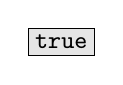
\begin{tikzpicture}
      \node [bddterminal] {$\true$};
    \end{tikzpicture}}
\newcommand{\bddfalse}[0]{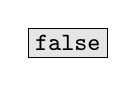
\begin{tikzpicture}
      \node [bddterminal] {$\false$};
    \end{tikzpicture}}


% Standardize command font styles and environments
\newcommand{\doccmd}[1]{\texttt{\textbackslash#1}}% command name -- adds backslash automatically
\newcommand{\docopt}[1]{\ensuremath{\langle}\textrm{\textit{#1}}\ensuremath{\rangle}}% optional command argument
\newcommand{\docarg}[1]{\textrm{\textit{#1}}}% (required) command argument
\newcommand{\docenv}[1]{\textsf{#1}}% environment name
\newcommand{\docpkg}[1]{\texttt{#1}}% package name
\newcommand{\doccls}[1]{\texttt{#1}}% document class name
\newcommand{\docclsopt}[1]{\texttt{#1}}% document class option name
\newenvironment{docspec}{\begin{quote}\noindent}{\end{quote}}% command specification environment



\begin{document}

\maketitle% this prints the handout title, author, and date

This course is all about probabilistic programs. To make a course about
something, it has to be suitably important. What are probabilistic programs, and
what makes them worth studying?  In short, \defn{probabilistic
programming languages} (PPLs) use the syntax and semantics of programs to define probability
distributions.\sidenote{\textbf{Syntax} is a textual representation of a program. \textbf{Semantics} tells us 
what a program means. We will see more about these in later lectures.}
In a typical programming language -- like OCaml, Python, or C -- 
a program's execution is deterministic: program outputs are fully determined by inputs 
(and perhaps an environment). For instance, the following tiny program 
produces an output of 15:\sidenote{Throughout the class and in these notes, we will use 
functional ML-style syntax for programs.}

\begin{lstlisting}
let x = 5 in
let y = 10 in
x + y
\end{lstlisting}

Probabilistic programs define probability distributions on their outputs. 
To do this, they have extra syntax and semantics for introducing and manipulating 
uncertain quantities. For instance, the following tiny probabilistic program flips 
two coins and returns the value \texttt{true} if both coins are heads:\sidenote{The syntax 
\texttt{flip }$\theta$ produces a random Boolean value that is \texttt{true} with probability $\theta$ 
and \texttt{false} with probability $1-\theta$.}

\begin{lstlisting}
let x = flip 0.5 in
let y = flip 0.5 in
x && y
\end{lstlisting}

This probabilistic program does not output a single value like \texttt{true} or
\texttt{false}: rather, it outputs a \emph{probability distribution} over all
the possible output values. In this case, it outputs the following \defn{probability 
distribution}, which is a function that associates values with probabilities:
\begin{align*}
  [\texttt{true} \mapsto 0.25, \qquad \texttt{false} \mapsto 0.75].
\end{align*}

Why would one want programs that manipulate probabilities in this way,
and what are the challenges that come along with this significant enrichment of
our usual programming model? 
There are many reasons, and today PPLs are a vibrant area of active research and 
development, but there is one theme in particular that I aim to explore in this course:
that \emph{PPLs are best understood as a cross-disciplinary 
effort between programming languages and artificial intelligence}.
This is because 
many of the motivations and methods necessary for designing, building, and studying PPLs stem from core 
research questions and methods studied from both of these areas.
In the following sections, we will explore 
this intersection, and survey some of the modern topics in PPL research that 
we will encounter during this course.

\section{The Programming Languages Perspective}

% \begin{marginfigure}
%   \centering
%   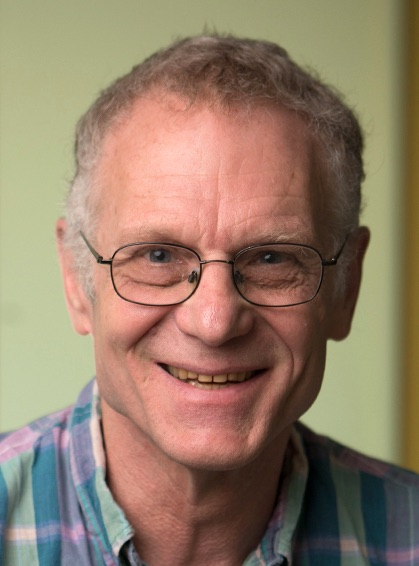
\includegraphics[width=50px]{graphics/kozen.jpeg}
%   \caption{Dexter Kozen. }
% \end{marginfigure}
% \begin{quote}
% ``Probabilistic computation has recently become an important topic of investigation
%   in theoretical computer science.'' \citet{kozen1979semantics}
% \end{quote}

Our first collection of answers to the question of ``why probabilistic
programming languages'' comes from formal study and application of programming
languages. One of the main goals of programming language research is to develop
programming languages foundations that enable the practical development of
robust and reliable software systems. Here is a small collection of some 
of the themes and success stories within programming languages towards this goal over the past
decades:

\begin{itemize}
  \item \emph{Deductive verification} and proof systems that verify that 
  programs satisfy certain specifications by the application of proof 
  rules that reason abstractly about program's behavior. Examples include the weakest
  pre-condition calculus and Hoare logic, separation logic, refinement logics, etc. 
  These techniques are typically not fully automated and require some sort of 
  guidance from the user in order to be applied.
  \item \emph{Type systems} that verify that programs satisfy certain
  properties. Type systems range broadly in sophistication. Some type systems 
  embed entire program logics~\citep{jhala2021refinement}. Others are more lightweight.
  Almost all programmers today interact with some form of type system while 
  writing their software.
  \item \emph{Semantic foundations}. How do we formally specify what it means to ``run a program''? 
  Can we associate programs with more abstract mathematical objects that are easier to 
  reason about? These are core questions within programming language research that fall under 
  the category of semantics, and the area is surprisingly deep: it can be difficult to precisely 
  describe what it means to execute a program.\sidenote{See \citet{pierce2002types} Chapter 3 for a 
  discussion the different kinds of semantics that have been investigated for programs.}
  \item \emph{Software model checking} that statically verify that programs satisfy 
  certain properties by somehow representing the entire state space of the program.
  Common techniques used in this area are SAT/SMT solvers such as Z3~\citep{de2008z3}
  and bounded model checking.
  % \item \emph{Correct by construction} software. 
\end{itemize}

These techniques are applied broadly in industry in places like NASA~\citep{calcagno2015moving}, 
Facebook~\citep{distefano2019scaling}, Microsoft~\citep{ball2004slam}, Amazon~\citep{newcombe2015amazon}, and 
many others.

\newthought{However, there is a fundamental problem}: what happens when the 
software system you want to reason about has \emph{inherent uncertainty} in it?
When you look hard enough for it, you
encounter uncertainty in almost every sufficiently large software system:
\begin{enumerate}
  \item \emph{Interaction with the environment}. The world is complicated and 
  software often has to interact with it.
  Hardware can fail randomly, physical processes (like turbulant flow)
  are computationally intractable to precisely model, and sometimes software has
  to interact with human beings. All these situations involve inherent
  uncertainty that software systems need to be able to deal with robustly.
  \item \emph{Randomized algorithms}. Some algorithms only output correct 
  answers with a certain probability~\citep{motwani1995randomized}. If we want to verify that an
  implementation of these algorithms is correct, we need to be able to 
  formally reason about programs with uncertain outcomes.\sidenote{Verification of 
  randomized algorithms was the original context in which \citet{kozen1979semantics} proposed 
  the study of giving a formal semantic foundation to probabilistic programs.}
  \item \emph{Machine learning}. Today, not all aspects of programs are written down as code: 
  often a program's behavior is determined by components that are learned from data. Machine 
  learning is riddled with uncertainty: both the learning process and the prediction process 
  are inherently uncertain processes. 
\end{enumerate}

The net result is that, in order to verify and formally reason about today's
software systems, we often need to reason about uncertainty. 
This requires revisiting each of the above research themes: weakest pre-condition 
calculus becomes weakest pre-expectation calculus~\citep{mciver2005abstraction},
model checking becomes probabilistic model checking~\citep{katoen2016probabilistic},
semantic foundations must incorporate probabilities~\citep{kozen1979semantics},
and so on.
In short, PPL research within the programming languages community has been
animated by a motivation to handle the need of reasoning formally about the
uncertainty that naturally arises in software systems.

\section{The Artificial Intelligence Perspective}
One of the main intellectual endeavors within artificial intelligence is the 
design and implementation of intelligent agents that reason rationally about their environments.
This inherently requires reasoning about uncertainty, an within the AI 
community there has been an enormous effort to scale, automate, and productize 
systems for automatically reasoning about uncertainty.\sidenote{There is even 
a major conference focusing on this problem called \emph{Uncertainty in 
Artificial Intelligence (UAI).}}
Within the AI community, these tools are broadly known as \emph{probabilistic models}.

A \defn{probabilistic model} is a language for describing a probability distribution.
The most popular and widely-known probabilistic model within the AI community is
the \emph{probabilistic graphical model} (PGM), a graphical representation of
uncertainty introduced by \citet{pearl1988probabilistic}.\sidenote{Several good
textbooks on PGMs have been written in recent years, including
\citet{darwiche2009modeling} and \citet{koller2009probabilistic}.} PGMs use 
graphical notation to describe the relationships between random quantities. 
For instance, the relationship ``if it is raining, then the ground is likely 
to be wet'' can be represented graphically as:
\begin{center}
  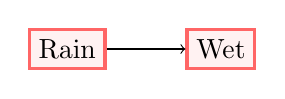
\begin{tikzpicture}[
    roundnode/.style={circle, draw=green!60, fill=green!5, very thick, minimum size=7mm},
    squarednode/.style={rectangle, draw=red!60, fill=red!5, very thick, minimum size=5mm},
    ]
    %Nodes
    \node[squarednode]      (maintopic)                              {Rain};
    \node[squarednode]      (rightsquare)       [right=of maintopic] {Wet};
    
    %Lines
    \draw[->] (maintopic.east) -- (rightsquare.west);
    \end{tikzpicture}
\end{center}

The directed edges denote dependencies: the fact that it is wet is statistically 
dependent on whether or not it is raining. The above is an example of a \emph{directed 
graphical model} or \emph{Bayesian network}.\sidenote{There are other kinds of graphical 
models that are undirected, such as factor graphs and Markov networks.}
Seen from this vantage point, probabilistic programming languages are a natural
evolution of existing graphical languages for representing uncertainty; indeed,
many early PPL papers explicitly reference this
lineage~\citep{sato1997prism,ramsey2002stochastic,goodman2012church}.


Concretely, we can represent the above rain--wet scenario using a simple
probabilistic program:

\begin{lstlisting}
let rain = flip 0.01 in
let wet = if rain then flip 0.9 else flip 0.01 in
wet
\end{lstlisting}

This program expresses that, on a given day, there is a 1\% chance that it is 
raining. In the event that it rains, then it is wet 90\% of the time; 
if it is not raining, then it is wet 1\% of the time. The program then outputs 
the variable that indicates whether or not it is wet. Notice how, rather than 
use a graph structure to describe relationships between uncertain quantities, 
a PPL uses standard programming constructs (such as \texttt{if}-statements).

\newthought{What do AI researchers} use probabilistic models for? One of the 
primary applications is \emph{Bayesian learning}. AI researchers want to 
design intelligent agents that reason rationally about their environment. A 
core part of this process is the ability to incorporate new information into 
the agent's model of the world as it is discovered. As a very simple example of 
this process, suppose we observe that it is wet and wish to to infer 
what the probability is that it rained. This process of observing new information 
and updating our beliefs can be encoded directly into the program using 
an \texttt{observe} keyword:

\begin{lstlisting}
let rain = flip 0.01 in
let wet = if rain then flip 0.9 else flip 0.01 in
observe wet;
rain
\end{lstlisting}

This program \emph{does not} output the distribution $[\true \mapsto 0.01, \false \mapsto 0.99]$!
By observing that the ground was wet, we correspondingly increase our 
estimate of the probability that it rained. Intuitively, this is accomplished 
by discarding all possible program executions that violate the \texttt{observe}'s 
constraints: in this case, all paths in which \texttt{wet = \false} are discarded, and 
a new \emph{posterior probability} of \texttt{rain} is computed. The outputted posterior 
probability on \texttt{rain} is:
\begin{align*}
  \left[\true \mapsto \frac{0.01 * 0.9}{0.01 * 0.9 + 0.99 * 0.01}, \false \mapsto \frac{0.99 * 0.01}{0.01 * 0.9 + 0.99 * 0.01} \right]
\end{align*}
This process of updating beliefs is called \defn{Bayesian conditioning}, 
and we will discuss observation in more detail a later lecture.
Computing the posterior probability of an event is called \defn{Bayesian inference}.\sidenote{As a 
preview, you have probably seen the rule for Bayes's rule before. Let 
$\Pr(X,Y)$ be a probability distribution on two random variables $X$ and $Y$. 
Then, the posterior probability of $X$ given $Y=y$ is:
$$\Pr(X = x \mid Y=y) = \frac{\Pr(X = x, Y = y)}{\Pr(Y=y)}.$$}

This ability to update our beliefs is critical for many AI applications 
that involve probabilistic reasoning:
\begin{itemize}
  \item \emph{Medical diagnosis}. A doctor posits the relationships between symptoms and 
  diseases, and wishes to infer the posterior probability of disease given observations 
  of symptoms.
  \item \emph{Image processing}. One assumes an underlying generative model of images, 
  observes a particular image, and infers the posterior probability on features of the 
  generative model. This has been used for infilling, denoising, and other forms of image processing.
  \item \emph{Game playing}. Many kinds of games involve \emph{imperfect information}: players
  don't get to know everything about each other. In imperfect information games, in order to 
  play optimally, it is necessary to infer aspects of the other player's state given observations 
  about their actions.
  \item \emph{Error correcting codes}. Today's software and hardware systems need to be robust to 
  events that randomly corrupt data. The problem of recovering possibly corrupted data can 
  be formulated as a Bayesian inference problem.
\end{itemize}
There are many more applications than listed here. Think of some for yourself!

\section{Modern Research Directions \& Challenges}
We have seen two very different avenues that arrive at the same destination: 
probabilistic programming languages are well-motivated from both an AI and PL 
perspective.  So, at this point you should be asking: if probabilistic
programming languages are so great and useful, why isn't everyone using them? 
Now we will survey some of the modern challenges in building practical PPLs 
that we will encounter during this course.


% Now I will briefly survey several of the modern research directions that drive
% current efforts to create effective probabilistic programming languages and
% systems.
% \begin{itemize}
%   \item Programming Languages Design and Implementation (PLDI)
% \end{itemize}

\begin{itemize}
  \item \emph{Hardness of inference}. The first and perhaps primary challenge
  for building practically useful PPLs is the fundamental computational
  complexity of probabilistic inference. We will see that, even for extremely 
  restricted languages, inference will be worst-case computationally intractable. 
  This means that all PPLs walk a delicate line between \emph{expressivity and
  tractability}: a more expressive language gives the user more freedom to write 
  programs, but makes the inference task correspondingly harder. To address this,
  PPL researchers develop inference strategies that identify and exploit various kinds 
  of program structure, such as independences, smoothness, unimodality, and other kinds of
  structure; we will see much more on this later in the course.

  \item \emph{Semantic foundations}. PPLs give the user an incredible amount of 
  flexibility in defining probability distributions: programs may have recursion, 
  conditioning, higher-order functions, etc. Formally reasoning about probability 
  distributions on these objects is very hard! We will encounter this in more detail 
  when we start writing down formal semantics for languages in later lectures.

  \item \emph{Deductive verification}. One way around the computational complexity 
  of inference is to reason about what probabilistic 
  programs do \emph{without running them}: this is the goal of deductive verification 
  strategies that aim to give proof rules for reasoning about probabilistic 
  programs. Deductive verification is an active area of PPL research that we will 
  explore in later lectures.
\end{itemize}

This is just a sample of some of the modern ongoing areas of research within PPLs 
today. To see more, check out some of the following research venues that regularly 
publish PPL papers:
\begin{itemize}
  \item Programming Language Design and Implementation (PLDI)
  \item Uncertainty in Artificial Intelligence (UAI)
  \item Symposium on Programming Languages (POPL)
  \item Object-oriented Programming Languages \& Applications (OOPSLA)
  \item Workshop on Languages for Inference (LAFI)
  \item Neural Information Processing Symposium (NeurIPS)
\end{itemize}

\bibliography{../bib}
\bibliographystyle{plainnat}



\end{document}
